\documentclass{beamer}
\usepackage[utf8]{inputenc}
\usetheme{Warsaw}  %% Themenwahl
\usepackage{algpseudocode}
\usepackage{algorithm}

\usepackage{mathtools}
\usepackage{tikz}
\usepackage{hyperref}
\usepackage{inputenc}
\usepackage{romannum}
\usepackage{longtable}
\newcommand{\specialcell}[2][c]{%
	\begin{tabular}[#1]{@{}c@{}}#2\end{tabular}}

\usepackage[T1]{fontenc}
\usepackage{selinput}
\SelectInputMappings{
	adieresis={ä},
	germandbls={ß}
}
\usepackage{babel}
\usepackage{ulem}
\usepackage{animate}

\title{Simulation And Optimization Of Traffic Light}
\author{Öztürk Emrah, Nicolai Schwartze, Jan Wenger}
\date{\today}
\usepackage{amssymb}
\usepackage{float}
\usepackage{cancel}

\begin{document}
	\maketitle
	%\frame{\tableofcontents[currentsection]}
	
	\section{Introduction}
	\frame{\tableofcontents[currentsection]}
	%\frame{\tableofcontents[currentsection]}
	\begin{frame}
		optimization of fairness, stop time and number of stops

		\begin{equation*}\label{key}
		func = \frac{g_{1}fairness + g_{2}stop\textunderscore time+g_{3}number\textunderscore stops}{3}\rightarrow \min
		\end{equation*}
		
		\begin{figure}[H]
			\centering
			\includegraphics[width=0.7\linewidth]{"sumo2"}
			%\caption{simulation in sumo}
			\label{fig:sumo2}
		\end{figure}
	\end{frame}

	\begin{frame}
	\frametitle{Simplifications}
		\begin{itemize}
			\item simplifications of software SUMO
			\item velocity, gap between cars and acceleration same
			\item one constant input stream from every geographic direction (N,S,W,E)
			\item perfection = 1, same turn probabilities (0.5 straight ahead, 0.25 left and right)
			\item one type of car, non intelligent, dynamic rerouteing
			\item exponential distribution for input streams
			\item stop simulation after 3600 simulation steps
		\end{itemize}
		
	\end{frame}
	
%	\begin{frame}
%	\frametitle{Differential Evolution}
%		
%	mutation operator
%	\begin{equation*}\label{key}
%	v_{i} = x_{r1} + F(x_{r2}-x_{r3})
%	\end{equation*}
%	
%	crossover operator
%	\begin{equation*}
%	u_{ij}=\begin{cases}
%	v_{ij}, &\text{if $j = K \lor rand[0,1] \leq CR$}\\
%	x_{ij}, &\text{otherwise}
%	\end{cases}
%	\end{equation*}
%
%	\end{frame}

	\section{Scenario/Program}
	\frame{\tableofcontents[currentsection]}
	
	\begin{frame}
		
		%\begin{itemize}
		%	\item night epsilon = 0.9
		%	\item day epsilon = 0.5
		%	\item Hill Climbing, Conjugate Gradient Descent,  %		NSGA-II,Differential Evolution
		%\end{itemize}
		
		\begin{figure}[H]
			\centering
			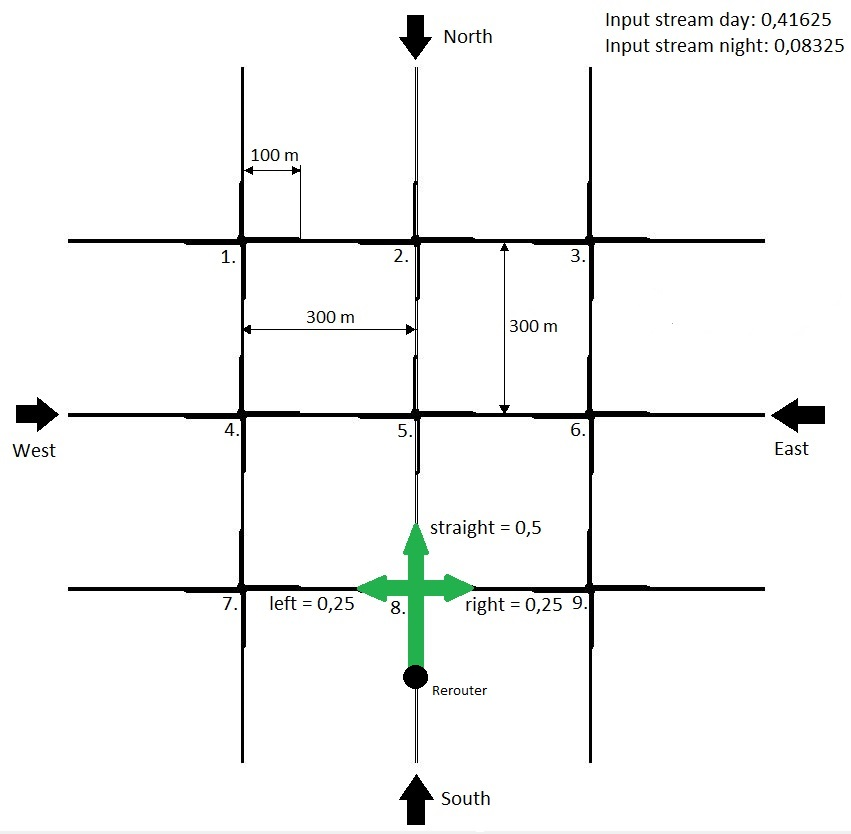
\includegraphics[width=0.7\linewidth]{3x3_inf}
			\label{fig:3x3inf}
		\end{figure}
	\end{frame}
	
	\begin{frame}
		\begin{figure}[H]
			\centering
			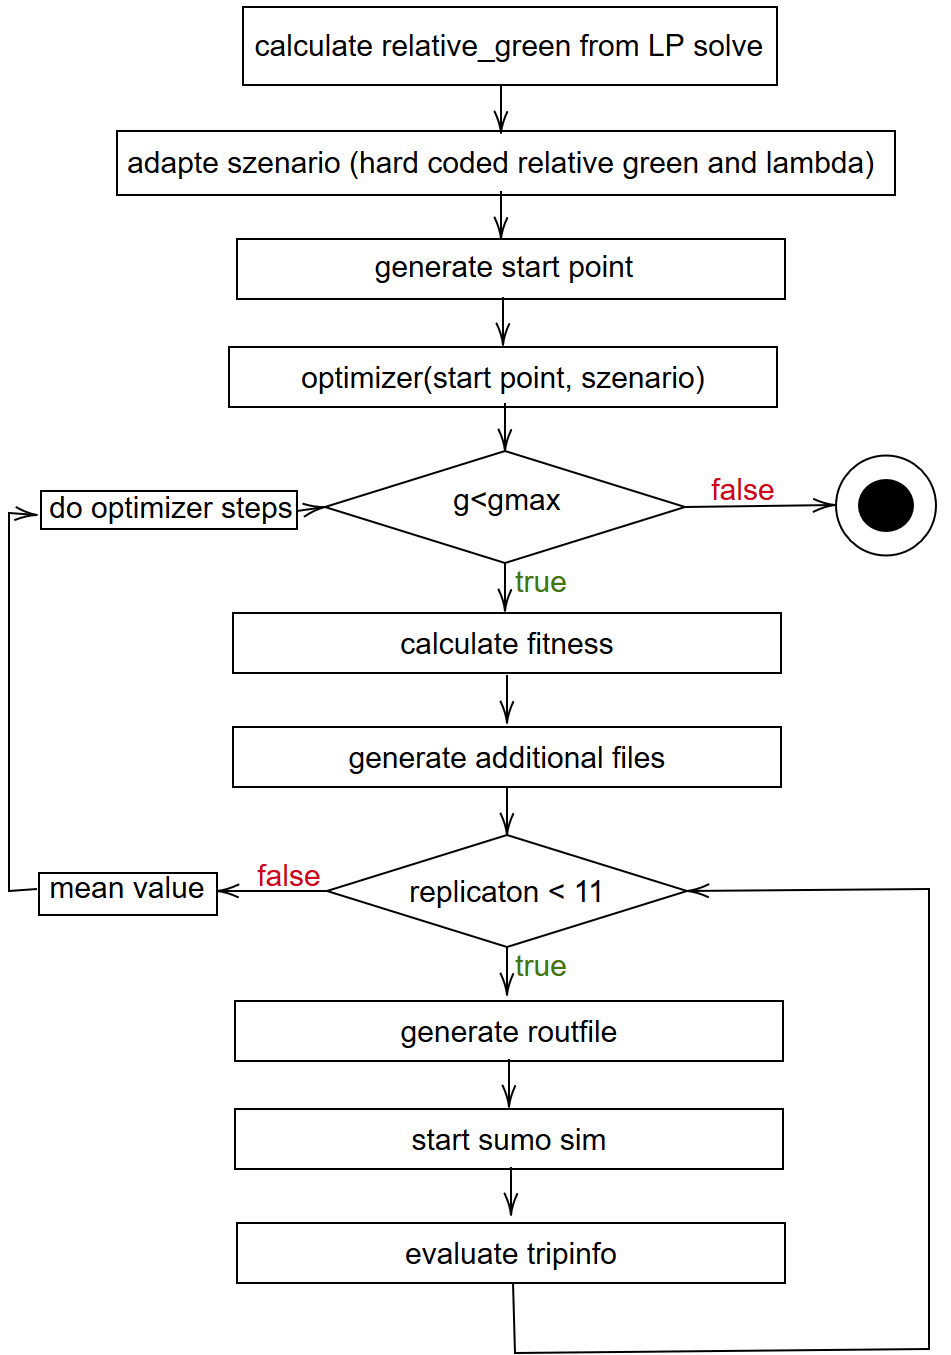
\includegraphics[width=0.45\linewidth]{diagram-202001222}
			\label{fig:diagram-202001222}
		\end{figure}
	\end{frame}

	\section{Optimization Algorithm}
	\frame{\tableofcontents[currentsection]}

	\begin{frame}
	\frametitle{Differential Evolution}
	\begin{algorithm}[H]{Differential evolution}
		\begin{algorithmic}[1]
			\State population $\leftarrow initialization$
			\State \textbf{while} $g<G_{max}$ \textbf{do}
			\State \ \ \ \ \textbf{for} individual $x_{i}$ \textbf{in} population \textbf{do}
			\State \ \ \ \ \ \ \ \ $v_{i}$ = mutation($x_{i}$, population,F)
			\State \ \ \ \ \ \ \ \ $u_{i}$ = crossover($x_{i},v_{i}$,CR)
			\State \ \ \ \ \ \ \ \ \textbf{if} function($u_{i}$) < function($x_{i}$) \textbf{then}
			\State \ \ \ \ \ \ \ \ \ \ \ \ $x_{i} = u_{i}$
			\State \ \ \ \ \ \ \ \ \textbf{end}
			\State \ \ \ \ \textbf{end}
			\State \ \ \ \ g = g + 1
			\State \textbf{end}
		\end{algorithmic}
	\end{algorithm}
		
	\end{frame}

	\begin{frame}
	\frametitle{NSGA-II}
		\begin{algorithmic}[1]
			\State population $\leftarrow initialization$
			\State \textbf{while} $g<G_{max}$ \textbf{do}
			\State \ \ \ \ \textbf{for} i \textbf{in} $\frac{population}{2}$ \textbf{do}
			\State \ \ \ \ \ \ \ \ $p_{1},p_{2}$ = tournament\textunderscore selection($P_{t}$)
			\State \ \ \ \ \ \ \ \ $q_{1},q_{2}$ = crossover($p_{1},p_{2}$)
			\State \ \ \ \ \ \ \ \ $q_{1}$ = mutations($q_{1}$)
			\State \ \ \ \ \ \ \ \ $q_{2}$ = mutations($q_{2}$)
			\State \ \ \ \ \ \ \ \ $Q_{t}$ = $Q_{t} \cup (q_{1},q_{2})$
			\State \ \ \ \ \textbf{end}
			\State \ \ \ \ $R_{t} = R_{t} \cup (Q_{t})$
			\State \ \ \ \ $R_{t}$ = fast\textunderscore non \textunderscore dominated \textunderscore sort($R_{t}$)
			\State \ \ \ \ $P_{t}$ = crowding\textunderscore distance \textunderscore sorting($R_{t},P_{t}.size$)
			\State \ \ \ \ g = g + 1
			\State \textbf{end}
		\end{algorithmic}
	\end{frame}

	\begin{frame}
	\frametitle{Conjugate Gradient Descent}
		\begin{algorithmic}[1]
			\State x,d $\leftarrow$ initialization
			\State \textbf{while} $||\nabla f(x)|| > \epsilon$ \textbf{or} ||$\hat{\eta}$d||<$\epsilon$\textbf{do}
			\State \ \ \ \ grad = numGrad(x)
			\State \ \ \ \ d = -grad + $\frac{||grad||^2}{||grad_{old}||^2d}$
			\State \ \ \ \ \textbf{if} $\frac{grad d}{||grad_{old}||||d||}>-\alpha$ \textbf{then}
			\State \ \ \ \ \ \ \ \ d = -grad
			\State \ \ \ \ \textbf{end}
			\State \ \ \ \ $\hat{\eta} = linsearch(f(x,d))$
			\State \ \ \ \ $x_{old} = x$ 
			\State \ \ \ \ $grad_{old}=grad$
			\State \ \ \ \ $x = x +\hat{\eta}d $
			\State \textbf{end}
		\end{algorithmic}
	\end{frame}

	\begin{frame}
	\frametitle{Hill Climbing}
	\begin{small}
		\begin{algorithmic}[1]
			\State $x_{start}$ $\leftarrow$ initialization
			\State \textbf{while} $fe<\#FE_{max}$ \textbf{do}
			\State \ \ \ \ \textbf{for} d \textbf{in} Dim \textbf{do}
			\State \ \ \ \ \ \ \ \ $z[d] = step$
			\State \ \ \ \ \ \ \ \ $y_{1,2} = x\pm step$
			\State \ \ \ \ \ \ \ \ $f = function(y)$
			\State \ \ \ \ \ \ \ \ $fe = fe + 1$
			\State \ \ \ \ \textbf{end}
			\State \ \ \ \ \textbf{if} function($y_{d}$)<function(x) \textbf{then} 
			\State \ \ \ \ \ \ \ \ $x = y_{d}$
			\State \ \ \ \ \textbf{end}
			\State \ \ \ \ \textbf{else}
			\State \ \ \ \ \ \ \ \ step = $\frac{step}{2}$
			\State \ \ \ \ \textbf{end}
			\State \textbf{end}
		\end{algorithmic}
	\end{small}
	\end{frame}
	
	

	\section{Experiments/Results}
	\frame{\tableofcontents[currentsection]}
	\begin{frame}
	\begin{longtable}{ | l | l |}
		\hline
		\raisebox{-\totalheight}{\animategraphics[loop,controls,width=0.8\linewidth]{1}{./exp_3x3_day_nsga2/nsga2_day_}{0}{19}}    &
		\raisebox{-\totalheight}{\specialcell{NSGA-II \\ parameter \\  $epsilon = 0.5$ \\ $pop size = 30 $ \\ $gen = 20 $}}\\
		\hline
	\end{longtable}	
	
		
	\end{frame}

	\begin{frame}
	
	\begin{longtable}{ | l | l |}
		\hline
		\raisebox{-\totalheight}{\animategraphics[loop,controls,width=0.8\linewidth]{1}{./exp_3x3_night_nsga2/nsga2_night_}{0}{14}}    &
		\raisebox{-\totalheight}{\specialcell{NSGA-II \\ parameter \\  $epsilon = 0.1$ \\ $pop size = 30 $ \\ $gen = 15 $}}\\
		\hline
	\end{longtable}	
		
	\end{frame}
	\begin{frame}
	\begin{longtable}{ | l | l |}
		\hline
		\raisebox{-\totalheight}{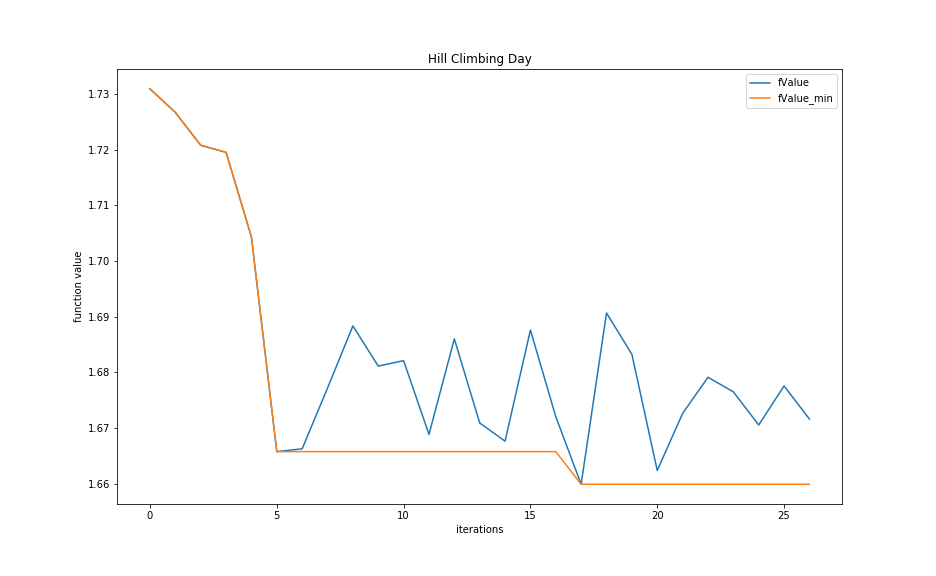
\includegraphics[width=\textwidth,height=0.7\textheight,keepaspectratio]{hc_day}}    &
		\raisebox{-\totalheight}{\specialcell{Hill-Climbing \\ parameter \\  $epsilon = 0.5$}}\\
		\hline
	\end{longtable}	
	\end{frame}

	\begin{frame}
		\begin{longtable}{ | l | l |}
			\hline
			\raisebox{-\totalheight}{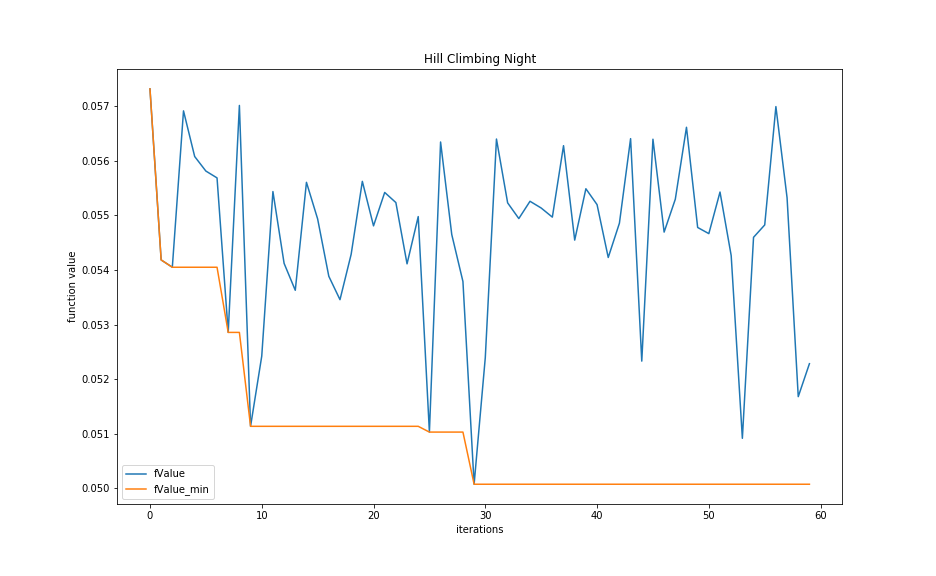
\includegraphics[width=\textwidth,height=0.7\textheight,keepaspectratio]{hc_night}}    &
			\raisebox{-\totalheight}{\specialcell{Hill-Climbing \\ parameter \\  $epsilon = 0.1$}}\\
			\hline
		\end{longtable}
	\end{frame}

	\begin{frame}
		\begin{longtable}{ | l | l |}
			\hline
			\raisebox{-\totalheight}{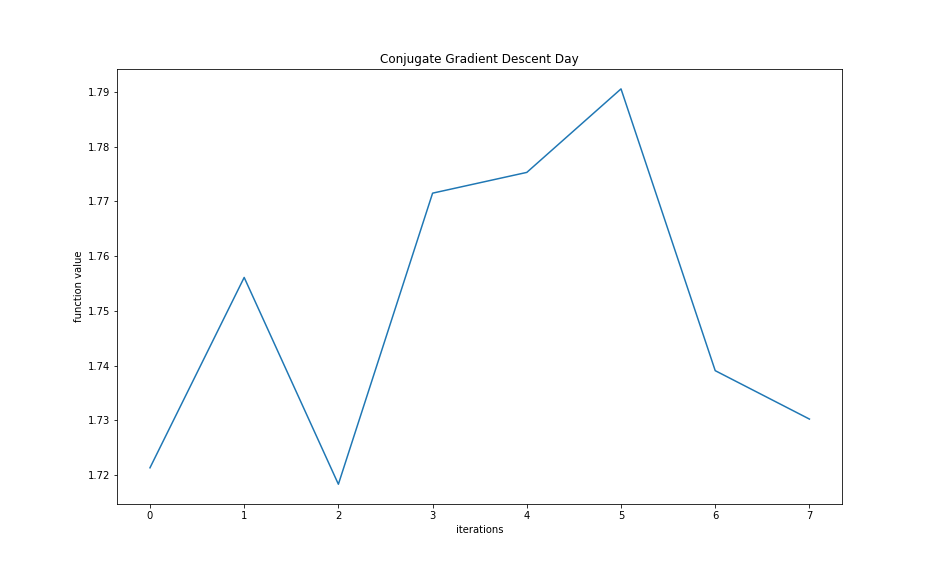
\includegraphics[width=\textwidth,height=0.7\textheight,keepaspectratio]{cgd_day}}    &
			\raisebox{-\totalheight}{\specialcell{Cgd \\ parameter \\  $epsilon = 0.5$ \\ $\alpha = 0.1$ \\ $\epsilon = 0.1$ \\ $\eta = 10 $ \\ $h = eps$}}\\
			\hline
		\end{longtable}	
	\end{frame}

	\begin{frame}
		\begin{longtable}{ | l | l |}
			\hline
			\raisebox{-\totalheight}{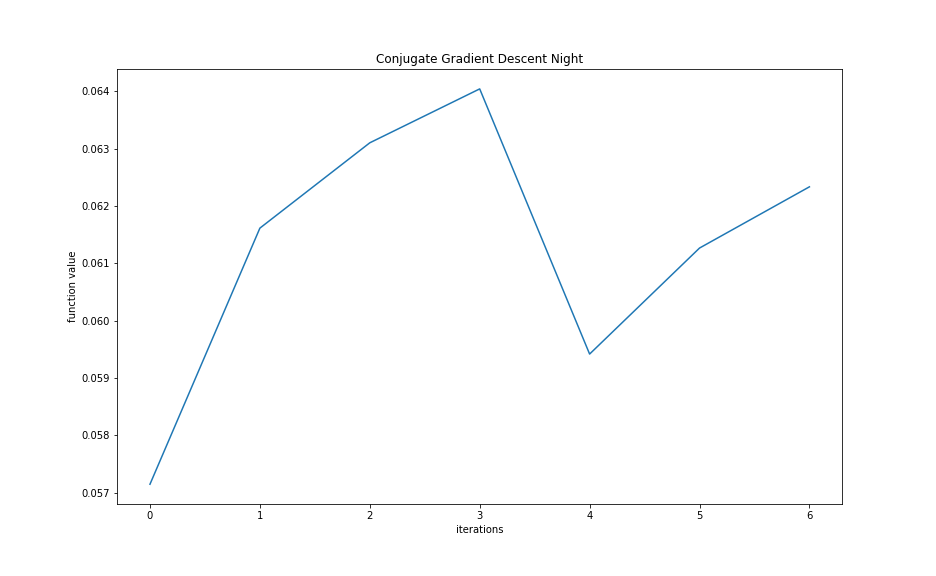
\includegraphics[width=\textwidth,height=0.7\textheight,keepaspectratio]{cgd_night}}    &
			\raisebox{-\totalheight}{\specialcell{Cgd \\ parameter \\  $epsilon = 0.1$ \\ $\alpha = 0.1$ \\ $\epsilon = 0.1$ \\ $\eta = 10 $ \\ $h = eps$}}\\
			\hline
		\end{longtable}	
	\end{frame}

	\section{Summary}
	\frame{\tableofcontents[currentsection]}
	
	\begin{frame}
		\frametitle{Summary}
		\begin{itemize}
			\item Problems:
			\begin{itemize}
				\item time consuming (calculation time)
				\item program crash (sumo)
				\item teleportation of cars
			\end{itemize}
			\item Reduction of the cost function is observable
			\item No possibility to check for correctness
			\item Less function evaluations $\rightarrow$ less calculation time needed
			\item Conjugate gradient descent problem with line-search (probability based rout file generation) 
		\end{itemize}
	\end{frame}
\end{document}